\documentclass[a4paper, 12pt]{article}
\usepackage[a4paper,top=1.5cm, bottom=1.5cm, left=1cm, right=1cm]{geometry}
\usepackage{cmap}					
\usepackage{mathtext} 				
\usepackage[T2A]{fontenc}			
\usepackage[utf8]{inputenc}			
\usepackage[english,russian]{babel}
\usepackage{multirow}
\usepackage{graphicx}
\documentclass{article}
\usepackage{listings}
\usepackage{xcolor}
\graphicspath{ {./images/} }
\usepackage{wrapfig}
\usepackage{tabularx}
\usepackage{float}
\usepackage{longtable}
\usepackage{hyperref}
\hypersetup{colorlinks=true,urlcolor=blue}
\usepackage[rgb]{xcolor}
\usepackage{amsmath,amsfonts,amssymb,amsthm,mathtools} 
\usepackage{icomma} 
\usepackage{euscript}
\usepackage{mathrsfs}
\usepackage{enumerate}
\usepackage{caption}
\usepackage{enumerate}
\usepackage{graphicx}
\usepackage{caption}
\usepackage{subcaption}
\usepackage[europeanresistors, americaninductors]{circuitikz}
\DeclareMathOperator{\sgn}{\mathop{sgn}}
\newcommand*{\hm}[1]{#1\nobreak\discretionary{}
	{\hbox{$\mathsurround=0pt #1$}}{}}
\title{\textbf{Лабораторная работа по float}}
\author{Моргулёв Илья}
\date{Октябрь 10, 2023}
\begin{document}
    \maketitle

    \section{Введение.}
        \begin{enumerate}
            \item \textbf{Цель работы.}
            Изучение скорости работы алгоритмов и сортировок с различной асимптотикой, сравнение теоретических сведений с практическими результатами. Изучение различных степеней оптимизации.
            \item \textbf{Задачи.}
            Задачи взяты с одноимённой лабораторной работы.
            \item \textbf{Сторонние функции} \newline
            \lstset {
        language=C++,
        backgroundcolor=\color{black!5}, 
        basicstyle=\footnotesize,
        }
        Время
        \begin{lstlisting}
    #include <chrono>
    double get_time() {
    return std::chrono::duration_cast<std::chrono::microseconds>
    (std::chrono::steady_clock::now().time_since_epoch()).count();
    }
        \end{lstlisting}
        \lstset {
        language=C++,
        backgroundcolor=\color{black!5}, 
        basicstyle=\footnotesize,
        }
        Рандомайзер
        \begin{lstlisting}
    #include <random>
    int rand_uns(int min, int max) {
    unsigned seed = std::chrono::steady_clock::now().time_since_epoch().count();
    static std::default_random_engine e(seed);
    std::uniform_int_distribution<int> d(min, max);
    return d(e);
    }
        \end{lstlisting}
        \end{enumerate}
    \section{Ход работы.}
    \begin{enumerate}
        \item[$1^0$] \textbf{Пузырёк и его товарищи.}
        Задача: рассмотреть несколько сортировок с квадратичной зависимостью, построить графики зависимости времени от длинны массива, доказать, что зависимость квадратична.
        Используемые сортировки: Пузырёк, Шейкер, Вставка.
            \begin{enumerate}
                \item \textbf{Пузырёк (Bubble Sort)} \newline
                Метод: сравнение двух соседних членов.
                \item \textbf{Шейкер (Shaker Sort)} \newline
                Метод: основан на пузырьке, ключевым отличием яыляется одновременное рассмотрение массива как слева-направо так и справа-налево.
                \item \textbf{Вставка(Insertion Sort)} \newline
                Метод: на каждом шаге алгоритма мы выбираем элемент массива и находим ему место для вставки. Условно говоря, двигаем отсортированную подпоследовательность в массиве до тех пор пока не отсортируем весь массив.\newline
            \end{enumerate}
        \newpage
        Построим графики зависимости времени от количества членов в массиве для всех трех типов сортировок. \newline
        \begin{figure}[h!]
            \centering
    		      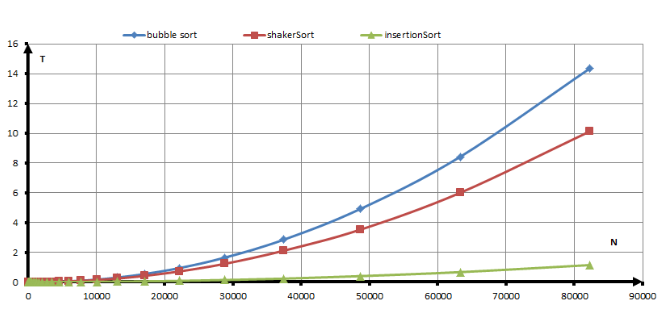
\includegraphics[scale = 0.8]{1.png}
    		      \caption{График зависимости Т(N)}
    		      \label{fig:my_label}
    	\end{figure}
        Докажем, что зависимость квадратична. Построим графики в логарифмических осях. \newline
        \begin{equation}
            T = \alpha N^2
        \end{equation}
        \begin{equation}
            \log T = \log \alpha N^2 = \log \alpha + \log N^2 = \textit{const} + 2\log N
        \end{equation}
        \begin{equation}
            \log T = C + 2\log N
        \end{equation}
        \begin{figure}[h!]
            \centering
    		      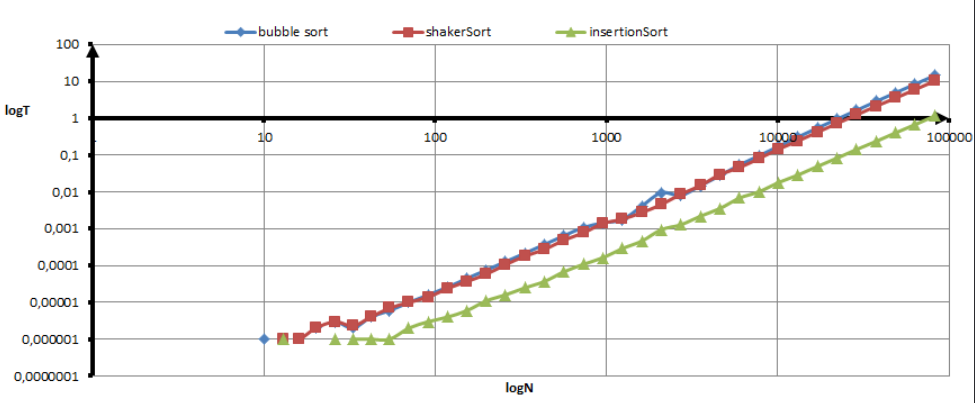
\includegraphics[scale = 0.55]{2.png}
    		      \caption{График зависимости $\log Т(\log N)$}
    		      \label{fig:my_label}
    	\end{figure} \newline
        Мы доказали, что сортировки, перечисленные выше действительно работают за $O(N^2)$
    \newpage
    \item[1.] \textbf{Пузырёк, но быстрее. Оптимизация}\newline
    Есть несколько различных вариантов оптимизации процессов: \newline
    $\textit{O}_0$ - самые простые и примитивные оптимизации\newline
    $\textit{O}_1$ - более сильные оптимизации\newline
    $\textit{O}_2$ - оптимизировать всё, что можно, но только проверенные и надёжные оптимизации\newline 
    $\textit{O}_3$ - жёсткая и насильственная оптимизация, применяются экспериментальные методы\newline
    Исследовать оптимизацию будем на Пузырьке. Ниже приведён график для зависимости времени от длины массива для разных типов оптимизации. \newline
    \begin{figure}[h!]
            \centering
    		      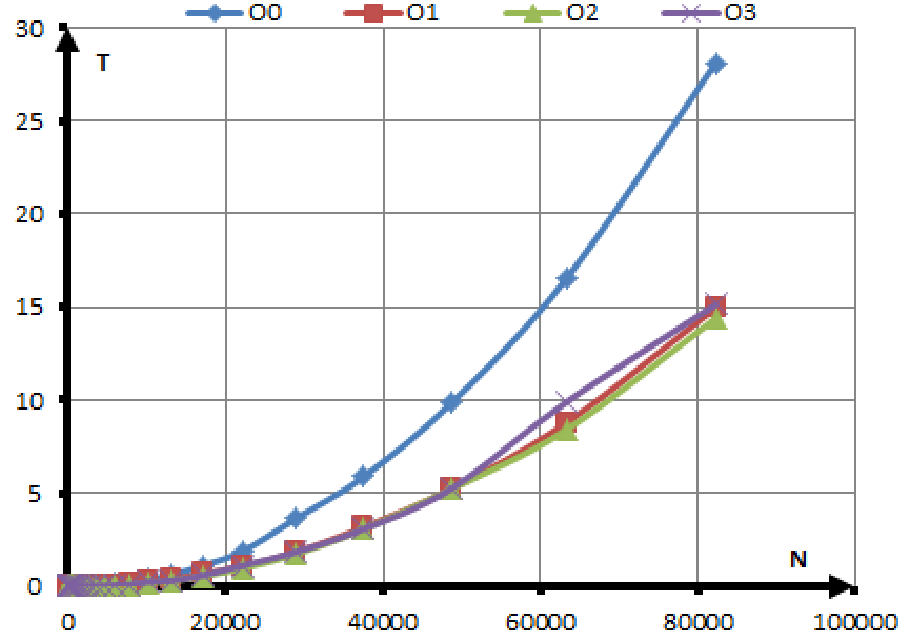
\includegraphics[scale = 0.55]{3.png}
    		      \caption{График зависимости T(N)}
    		      \label{fig:my_label}
    	\end{figure}
    На графике заметно, что $O_0$ заметно медленнее.

    \item[2] \textbf{А теперь настоящие быстрые сортировки.} \newline
    Ниже приведены сортировки, работающие за $O(N\log N)$, и кратко описаны алгоритмы их работы.
    \begin{enumerate}
        \item \textbf{Метод Слияние (Merge Sort)} \newline
        Разделяем массив на две половины и так делим, пока не получим подмассивы длины 1, потом каждые две половины сортируем между собой и объединяем. Повторяем до тех пор, пока весь массив не будет отсортирован.
        \item \textbf{Быстрая сортировка (Quick Sort)} \newline
        Выбираем в массиве некоторый элемент, который называется разрешающим. Затем он помещается в то место массива, где ему полагается быть после упорядочивания всех элементов. В процессе поиска подходящего места для разрешающего элемента производятся перестановки элементов так, что слева от них находятся элементы меньше разрешающего, а справа - больше.
        \item \textbf{Комбо Сортировка (Comb Sort)} \newline
        Изначально берёт большое расстояние между сравниваемыми элементами, в процессе сортировки сужая это расстояние. (Расчёска:)) \newline
        Отразим на графике время работы для этих сортировок. \newline
        \begin{figure}[h!]
            \centering
    		      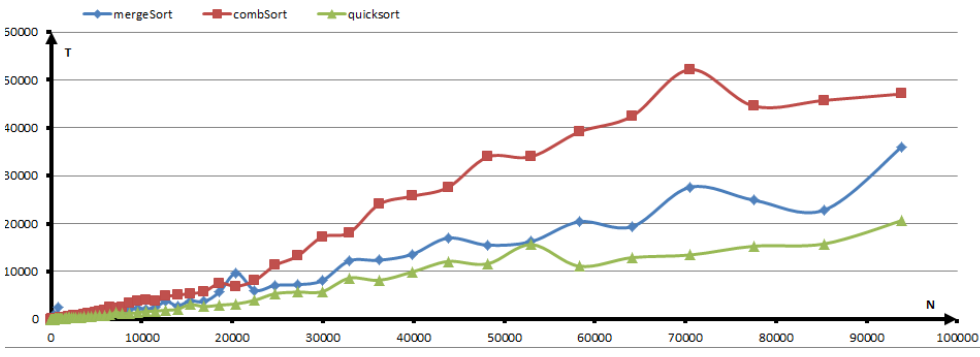
\includegraphics[scale = 0.55]{4.png}
    		      \caption{График зависимости T(N)}
    		      \label{fig:my_label}
    	\end{figure}
        \[\]
        Докажем, что эти сортировки действительно работают за $O(N\log N)$ \newline
        \begin{equation}
            T = \alpha N \log N
        \end{equation}
        \begin{equation}
            \alpha = \frac{T}{N \log N} \approx \textit{const}
        \end{equation}
        \begin{figure}[h!]
            \centering
    		      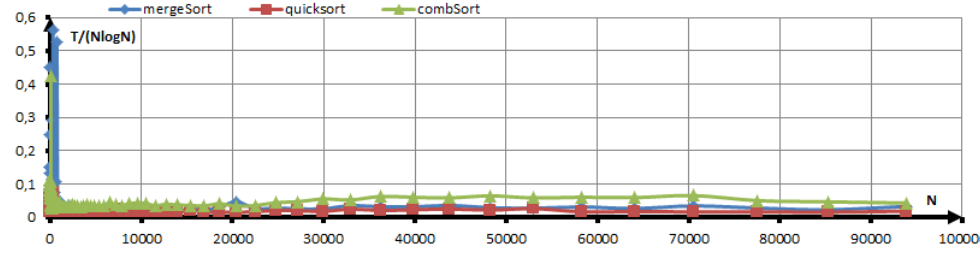
\includegraphics[scale = 0.55]{5.png}
    		      \caption{График зависимости $\alpha(N)$}
    		      \label{fig:my_label}
    	\end{figure}
        \[\]
        Мы доказали, что эти сортировки действительно работают за $O(N \log N)$        
    \end{enumerate}
    \newpage
    \item[3.] \textbf{$O(N^2)$ vs $O(N\log N)$} \newline
    Отразим на одном графике зависимоти от времени для всех ранее описанных сортировок. \newline
    \begin{figure}[h!]
            \centering
    		      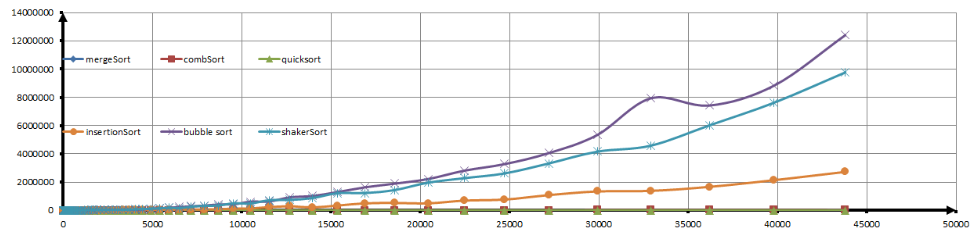
\includegraphics[scale = 0.55]{6.png}
    		      \caption{График зависимости T(N)}
    		      \label{fig:my_label}
    	\end{figure}
    \[\]
    Наглядно видно, что квадратичные сортировки работают кратно дольше.

    \item[4.] \textbf{Зависимость от начальных данных} \newline
    Рассмотрим, что будет происходить с зависимостями, если сортировки работают с уже отсортированным массивом (BEST), массиве рандомных чисел (GOOD) и массиве, отсортированном в обратном порядке (BAD).
    \begin{enumerate}
        \item \textcolor{blue}{\textbf{Пузырёк}}
            \begin{figure}[h!]
            \centering
    		      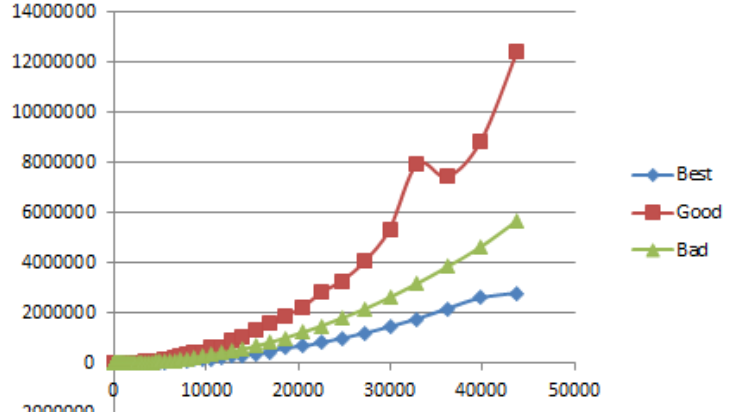
\includegraphics[scale = 0.55]{7.png}
    		      \caption{Три случая для Пузырька}
    		      \label{fig:my_label}
    	\end{figure}
    \newpage
        \item \textcolor{blue}{\textbf{Шейкер}}
    \begin{figure}[h!]
            \centering
    		      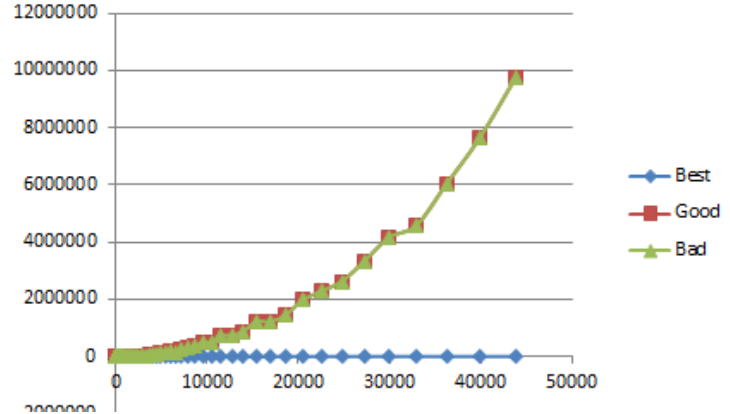
\includegraphics[scale = 0.55]{8.png}
    		      \caption{Три случая для Шейкера}
    		      \label{fig:my_label}
    	\end{figure}
        \item \textcolor{blue}{\textbf{Вставка}}
    \begin{figure}[h!]
            \centering
    		      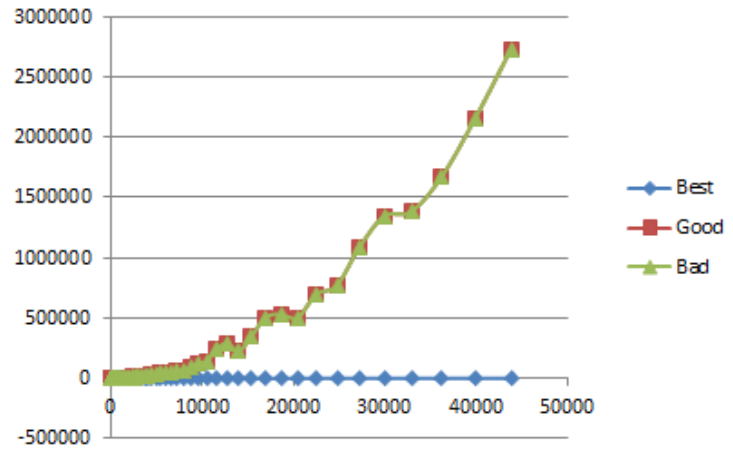
\includegraphics[scale = 0.55]{9.png}
    		      \caption{Три случая для Вставка}
    		      \label{fig:my_label}
    	\end{figure}
    \newpage
        \item \textcolor{blue}{\textbf{Выбор}}
    \begin{figure}[h!]
            \centering
    		      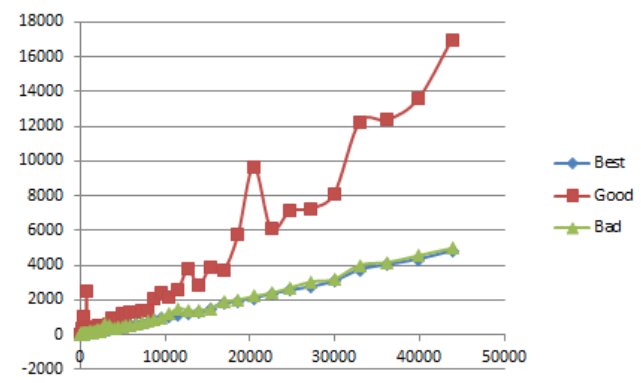
\includegraphics[scale = 0.55]{10.png}
    		      \caption{Три случая для Выбора}
    		      \label{fig:my_label}
    	\end{figure}
        \item \textcolor{blue}{\textbf{Расчёска}}
    \begin{figure}[h!]
            \centering
    		      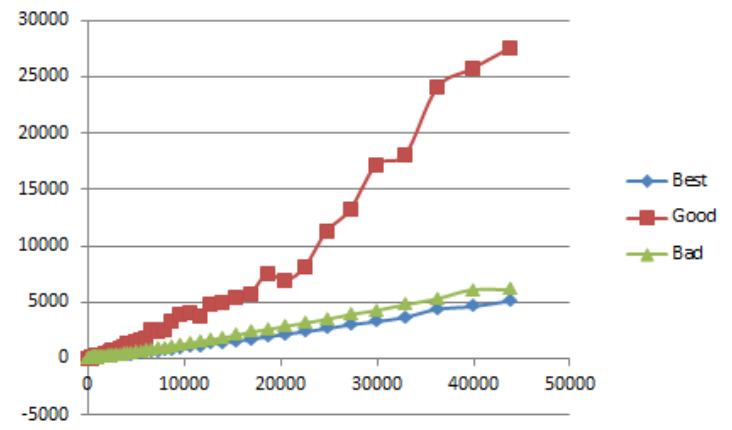
\includegraphics[scale = 0.55]{11.png}
    		      \caption{Три случая для Расчёски}
    		      \label{fig:my_label}
    	\end{figure}
    \newpage
        \item \textcolor{blue}{\textbf{Быстрая}}
    \begin{figure}[h!]
            \centering
    		      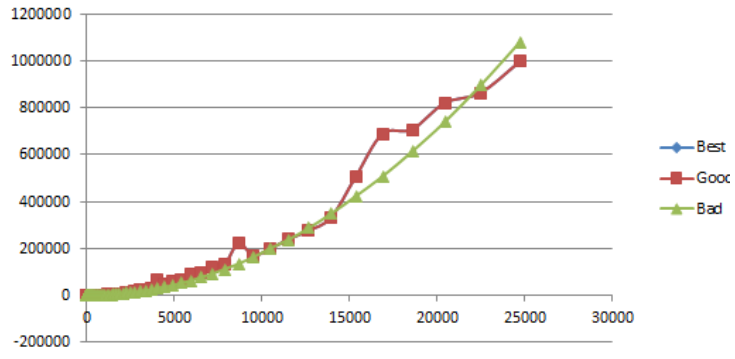
\includegraphics[scale = 0.55]{12.png}
    		      \caption{Три случая для Быстрой}
    		      \label{fig:my_label}
    	\end{figure}
    \end{enumerate}

    \item[4.] \textbf{Сравнение всех сортировок.} \newline
    Изобразим на одном графике последние шесть зависимостей (да, безумие, 18 зависимостей на одном графике))\newline
    \begin{figure}[h!]
            \centering
    		      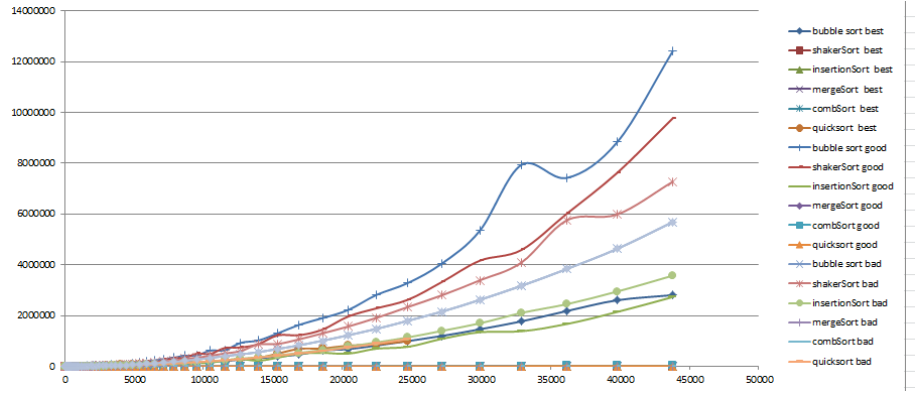
\includegraphics[scale = 0.55]{13.png}
    		      \caption{Общее}
    		      \label{fig:my_label}
    	\end{figure}
    \end{enumerate}
    \section{Вывод.}
    Мы рассмотрели различные типы сортировок и на деле убедились в верных оценках асимптотики их зависимостей.
\end{document}
